% Options for packages loaded elsewhere
\PassOptionsToPackage{unicode}{hyperref}
\PassOptionsToPackage{hyphens}{url}
%
\documentclass[
]{article}
\usepackage{amsmath,amssymb}
\usepackage{iftex}
\ifPDFTeX
  \usepackage[T1]{fontenc}
  \usepackage[utf8]{inputenc}
  \usepackage{textcomp} % provide euro and other symbols
\else % if luatex or xetex
  \usepackage{unicode-math} % this also loads fontspec
  \defaultfontfeatures{Scale=MatchLowercase}
  \defaultfontfeatures[\rmfamily]{Ligatures=TeX,Scale=1}
\fi
\usepackage{lmodern}
\ifPDFTeX\else
  % xetex/luatex font selection
\fi
% Use upquote if available, for straight quotes in verbatim environments
\IfFileExists{upquote.sty}{\usepackage{upquote}}{}
\IfFileExists{microtype.sty}{% use microtype if available
  \usepackage[]{microtype}
  \UseMicrotypeSet[protrusion]{basicmath} % disable protrusion for tt fonts
}{}
\makeatletter
\@ifundefined{KOMAClassName}{% if non-KOMA class
  \IfFileExists{parskip.sty}{%
    \usepackage{parskip}
  }{% else
    \setlength{\parindent}{0pt}
    \setlength{\parskip}{6pt plus 2pt minus 1pt}}
}{% if KOMA class
  \KOMAoptions{parskip=half}}
\makeatother
\usepackage{xcolor}
\usepackage[margin=1in]{geometry}
\usepackage{color}
\usepackage{fancyvrb}
\newcommand{\VerbBar}{|}
\newcommand{\VERB}{\Verb[commandchars=\\\{\}]}
\DefineVerbatimEnvironment{Highlighting}{Verbatim}{commandchars=\\\{\}}
% Add ',fontsize=\small' for more characters per line
\usepackage{framed}
\definecolor{shadecolor}{RGB}{248,248,248}
\newenvironment{Shaded}{\begin{snugshade}}{\end{snugshade}}
\newcommand{\AlertTok}[1]{\textcolor[rgb]{0.94,0.16,0.16}{#1}}
\newcommand{\AnnotationTok}[1]{\textcolor[rgb]{0.56,0.35,0.01}{\textbf{\textit{#1}}}}
\newcommand{\AttributeTok}[1]{\textcolor[rgb]{0.13,0.29,0.53}{#1}}
\newcommand{\BaseNTok}[1]{\textcolor[rgb]{0.00,0.00,0.81}{#1}}
\newcommand{\BuiltInTok}[1]{#1}
\newcommand{\CharTok}[1]{\textcolor[rgb]{0.31,0.60,0.02}{#1}}
\newcommand{\CommentTok}[1]{\textcolor[rgb]{0.56,0.35,0.01}{\textit{#1}}}
\newcommand{\CommentVarTok}[1]{\textcolor[rgb]{0.56,0.35,0.01}{\textbf{\textit{#1}}}}
\newcommand{\ConstantTok}[1]{\textcolor[rgb]{0.56,0.35,0.01}{#1}}
\newcommand{\ControlFlowTok}[1]{\textcolor[rgb]{0.13,0.29,0.53}{\textbf{#1}}}
\newcommand{\DataTypeTok}[1]{\textcolor[rgb]{0.13,0.29,0.53}{#1}}
\newcommand{\DecValTok}[1]{\textcolor[rgb]{0.00,0.00,0.81}{#1}}
\newcommand{\DocumentationTok}[1]{\textcolor[rgb]{0.56,0.35,0.01}{\textbf{\textit{#1}}}}
\newcommand{\ErrorTok}[1]{\textcolor[rgb]{0.64,0.00,0.00}{\textbf{#1}}}
\newcommand{\ExtensionTok}[1]{#1}
\newcommand{\FloatTok}[1]{\textcolor[rgb]{0.00,0.00,0.81}{#1}}
\newcommand{\FunctionTok}[1]{\textcolor[rgb]{0.13,0.29,0.53}{\textbf{#1}}}
\newcommand{\ImportTok}[1]{#1}
\newcommand{\InformationTok}[1]{\textcolor[rgb]{0.56,0.35,0.01}{\textbf{\textit{#1}}}}
\newcommand{\KeywordTok}[1]{\textcolor[rgb]{0.13,0.29,0.53}{\textbf{#1}}}
\newcommand{\NormalTok}[1]{#1}
\newcommand{\OperatorTok}[1]{\textcolor[rgb]{0.81,0.36,0.00}{\textbf{#1}}}
\newcommand{\OtherTok}[1]{\textcolor[rgb]{0.56,0.35,0.01}{#1}}
\newcommand{\PreprocessorTok}[1]{\textcolor[rgb]{0.56,0.35,0.01}{\textit{#1}}}
\newcommand{\RegionMarkerTok}[1]{#1}
\newcommand{\SpecialCharTok}[1]{\textcolor[rgb]{0.81,0.36,0.00}{\textbf{#1}}}
\newcommand{\SpecialStringTok}[1]{\textcolor[rgb]{0.31,0.60,0.02}{#1}}
\newcommand{\StringTok}[1]{\textcolor[rgb]{0.31,0.60,0.02}{#1}}
\newcommand{\VariableTok}[1]{\textcolor[rgb]{0.00,0.00,0.00}{#1}}
\newcommand{\VerbatimStringTok}[1]{\textcolor[rgb]{0.31,0.60,0.02}{#1}}
\newcommand{\WarningTok}[1]{\textcolor[rgb]{0.56,0.35,0.01}{\textbf{\textit{#1}}}}
\usepackage{graphicx}
\makeatletter
\def\maxwidth{\ifdim\Gin@nat@width>\linewidth\linewidth\else\Gin@nat@width\fi}
\def\maxheight{\ifdim\Gin@nat@height>\textheight\textheight\else\Gin@nat@height\fi}
\makeatother
% Scale images if necessary, so that they will not overflow the page
% margins by default, and it is still possible to overwrite the defaults
% using explicit options in \includegraphics[width, height, ...]{}
\setkeys{Gin}{width=\maxwidth,height=\maxheight,keepaspectratio}
% Set default figure placement to htbp
\makeatletter
\def\fps@figure{htbp}
\makeatother
\setlength{\emergencystretch}{3em} % prevent overfull lines
\providecommand{\tightlist}{%
  \setlength{\itemsep}{0pt}\setlength{\parskip}{0pt}}
\setcounter{secnumdepth}{-\maxdimen} % remove section numbering
\ifLuaTeX
  \usepackage{selnolig}  % disable illegal ligatures
\fi
\IfFileExists{bookmark.sty}{\usepackage{bookmark}}{\usepackage{hyperref}}
\IfFileExists{xurl.sty}{\usepackage{xurl}}{} % add URL line breaks if available
\urlstyle{same}
\hypersetup{
  pdftitle={Data Preprocessing and Feature Engineering: Sassafras},
  pdfauthor={Samantha Harper},
  hidelinks,
  pdfcreator={LaTeX via pandoc}}

\title{Data Preprocessing and Feature Engineering: Sassafras}
\usepackage{etoolbox}
\makeatletter
\providecommand{\subtitle}[1]{% add subtitle to \maketitle
  \apptocmd{\@title}{\par {\large #1 \par}}{}{}
}
\makeatother
\subtitle{Capstone}
\author{Samantha Harper}
\date{20 November 2024}

\begin{document}
\maketitle

{
\setcounter{tocdepth}{2}
\tableofcontents
}
\section{Background}\label{background}

\subsection{Research Question}\label{research-question}

The research question is: Can we use machine learning algorithms to mine
SNPs to find gene or gene regions of interest between natural cultivars
(strains) of Sassafras?

\subsection{Hypothesis}\label{hypothesis}

Hypothesis: Underlying genes, as identified by SNPs, in Sassafras are
influenced by environmental factors because environmental pressure can
cause mutations to persist in a population that is unique to each area.

\subsection{Prediction}\label{prediction}

Prediction: Populations of Sassafras that are under high environmental
pressure are more likely to have many predictive SNPs due to
evolutionary influences.

\section{Methods}\label{methods}

The goals for data pre-processing and feature engineering were to
transform the VCF data into a format compatible with machine learning
algorithms and to apply some level of feature selection to prepare for
accurate results from the ML algorithms. The first step is to transform
the wide data into long data and out of VCF format, keeping only the
relevant data. Then normalization and centering should be applied to the
data. The data needs to be split into test and training sets, and
feature selection should remove lowly expressed genes only after the
data has been split. Then, cross validation can be used to help with
hyperparameter tuning and with our relatively small sample size.

\subsection{Preprocessing}\label{preprocessing}

The vcfR package was used to convert the VCF data to a tibble. The
metadata from the original study was then cleaned and joined with the
sample names, since the original dataset only contained a row for each
population, instead of for each sample. The DeSeq Object requires a very
specific matrix, so the metadata and the genetic data both had row names
set and compared to ensure the object would load correctly. Once the
DeSeq Object was created, a Variation Stabilizing Transformation was
applied. Since the read counts for genetic data vary wildly, it is
essential that some kind of transformation be applied. The `local' VST
was applied after comparing the four options and comparing the resulting
standard deviation and spread of the data.

\subsection{Feature Selection}\label{feature-selection}

Before any feature selection, the data was split into test and training
sets to prevent data leakage. Principal Component Analysis (PCA) was
applied to the data. PCA is used to reduce the dimensionality of the
data and therefore help highlight important features. The PCA strategies
that were used didn't seem to fit the numerical nature of the data, and
an alternative will be considered before modelling.

\subsubsection{Results}\label{results}

\begin{Shaded}
\begin{Highlighting}[]
\CommentTok{\#Install packages and load library}

\NormalTok{pacman}\SpecialCharTok{::}\FunctionTok{p\_unload}\NormalTok{(pacman}\SpecialCharTok{::}\FunctionTok{p\_loaded}\NormalTok{(), }\AttributeTok{character.only =} \ConstantTok{TRUE}\NormalTok{)}
\end{Highlighting}
\end{Shaded}

\begin{verbatim}
## The following packages are a base install and will not be unloaded:
## 
\end{verbatim}

\begin{verbatim}
## The following packages were not previously loaded:
## 
\end{verbatim}

\begin{Shaded}
\begin{Highlighting}[]
\FunctionTok{rm}\NormalTok{(}\AttributeTok{list =} \FunctionTok{ls}\NormalTok{(}\AttributeTok{all =} \ConstantTok{TRUE}\NormalTok{))}

\NormalTok{pacman}\SpecialCharTok{::}\FunctionTok{p\_load}\NormalTok{(tidyverse,}
\NormalTok{               vcfR,}
\NormalTok{               ggplot2, }
\NormalTok{               kableExtra,}
\NormalTok{               BiocManager,}
\NormalTok{               DESeq2,}
\NormalTok{               pheatmap,}
\NormalTok{               RColorBrewer,}
\NormalTok{               vsn,}
\NormalTok{               gridExtra,}
\NormalTok{               ggrepel,}
\NormalTok{               e1071,}
\NormalTok{               caret,}
\NormalTok{               randomForest,}
\NormalTok{               ranger,}
\NormalTok{               multtest}
\NormalTok{)}
\end{Highlighting}
\end{Shaded}

\begin{Shaded}
\begin{Highlighting}[]
\CommentTok{\#Load VCF data}
\NormalTok{vcf }\OtherTok{\textless{}{-}} \FunctionTok{read.vcfR}\NormalTok{( }\StringTok{"Data/SNP.vcf"}\NormalTok{, }\AttributeTok{verbose =} \ConstantTok{FALSE}\NormalTok{ )}
\CommentTok{\#examine VCF object}
\NormalTok{vcf}
\end{Highlighting}
\end{Shaded}

\begin{verbatim}
## ***** Object of Class vcfR *****
## 106 samples
## 9177 CHROMs
## 11,862 variants
## Object size: 14.5 Mb
## 0 percent missing data
## *****        *****         *****
\end{verbatim}

\begin{Shaded}
\begin{Highlighting}[]
\CommentTok{\#Convert data to tibble}
\NormalTok{data }\OtherTok{\textless{}{-}} \FunctionTok{vcfR2tidy}\NormalTok{(vcf)}
\end{Highlighting}
\end{Shaded}

\begin{verbatim}
## Extracting gt element GT
\end{verbatim}

\begin{verbatim}
## Extracting gt element DP
\end{verbatim}

\begin{verbatim}
## Extracting gt element AD
\end{verbatim}

\begin{verbatim}
## Extracting gt element GL
\end{verbatim}

\begin{Shaded}
\begin{Highlighting}[]
\CommentTok{\#Isolate Counts Data}
\NormalTok{gdata }\OtherTok{\textless{}{-}}\NormalTok{ data}\SpecialCharTok{$}\NormalTok{gt}
\CommentTok{\#Load Metadata}
\NormalTok{sass\_metadata }\OtherTok{\textless{}{-}} \FunctionTok{read\_csv}\NormalTok{(}\StringTok{"Data/sass\_metadata.csv"}\NormalTok{, }\AttributeTok{col\_types =} \FunctionTok{cols}\NormalTok{(}\AttributeTok{Longitude =} \FunctionTok{col\_number}\NormalTok{(), }\AttributeTok{Latitude =} \FunctionTok{col\_number}\NormalTok{(), }\StringTok{\textasciigrave{}}\AttributeTok{Number of Samples}\StringTok{\textasciigrave{}} \OtherTok{=} \FunctionTok{col\_integer}\NormalTok{(), }\AttributeTok{Temperature =} \FunctionTok{col\_number}\NormalTok{(), }\AttributeTok{Precipitation =} \FunctionTok{col\_integer}\NormalTok{(), }\StringTok{\textasciigrave{}}\AttributeTok{Altitude (m)}\StringTok{\textasciigrave{}} \OtherTok{=} \FunctionTok{col\_integer}\NormalTok{()))}
\end{Highlighting}
\end{Shaded}

\begin{Shaded}
\begin{Highlighting}[]
\CommentTok{\#the goal is to have my matrix match the counts data from demo1}
\CommentTok{\#then I can feed the matrix into DeSeq2 and use the resulting counts}
\CommentTok{\#and hopefully those are correct?}
\NormalTok{gdata}\SpecialCharTok{$}\NormalTok{chrom\_info }\OtherTok{\textless{}{-}} \FunctionTok{paste}\NormalTok{(gdata}\SpecialCharTok{$}\NormalTok{ChromKey, }\StringTok{"\_"}\NormalTok{, gdata}\SpecialCharTok{$}\NormalTok{POS)}
\NormalTok{gdata }\OtherTok{\textless{}{-}}\NormalTok{ gdata }\SpecialCharTok{\%\textgreater{}\%} \FunctionTok{select}\NormalTok{(chrom\_info, Indiv, gt\_AD)}
\NormalTok{gdata }\OtherTok{\textless{}{-}}\NormalTok{ gdata }\SpecialCharTok{\%\textgreater{}\%} \FunctionTok{pivot\_wider}\NormalTok{(}\AttributeTok{names\_from =}\NormalTok{ Indiv, }\AttributeTok{values\_from =}\NormalTok{ gt\_AD)}
\end{Highlighting}
\end{Shaded}

\begin{Shaded}
\begin{Highlighting}[]
\CommentTok{\#set up matrix}
\NormalTok{gdata }\OtherTok{\textless{}{-}} \FunctionTok{as.data.frame}\NormalTok{(gdata)}
\FunctionTok{rownames}\NormalTok{(gdata) }\OtherTok{\textless{}{-}}\NormalTok{ gdata}\SpecialCharTok{$}\NormalTok{chrom\_info}
\NormalTok{gdata }\OtherTok{\textless{}{-}}\NormalTok{ gdata[ ,}\SpecialCharTok{{-}}\DecValTok{1}\NormalTok{]}
\end{Highlighting}
\end{Shaded}

\begin{Shaded}
\begin{Highlighting}[]
\CommentTok{\#create proper metadata}
\NormalTok{indivs }\OtherTok{\textless{}{-}} \FunctionTok{unique}\NormalTok{(data}\SpecialCharTok{$}\NormalTok{gt}\SpecialCharTok{$}\NormalTok{Indiv)}
\NormalTok{indivs }\OtherTok{\textless{}{-}} \FunctionTok{as.data.frame}\NormalTok{(indivs)}
\NormalTok{indivs}\SpecialCharTok{$}\NormalTok{id }\OtherTok{\textless{}{-}} \FunctionTok{substr}\NormalTok{(indivs}\SpecialCharTok{$}\NormalTok{indivs, }\DecValTok{1}\NormalTok{, }\DecValTok{2}\NormalTok{)}
\NormalTok{sass\_metadata}\SpecialCharTok{$}\NormalTok{id }\OtherTok{\textless{}{-}} \FunctionTok{substr}\NormalTok{(sass\_metadata}\SpecialCharTok{$}\NormalTok{Code, }\DecValTok{1}\NormalTok{, }\DecValTok{2}\NormalTok{)}
\NormalTok{joined\_meta }\OtherTok{\textless{}{-}} \FunctionTok{inner\_join}\NormalTok{(sass\_metadata, indivs, }\AttributeTok{by =} \StringTok{\textquotesingle{}id\textquotesingle{}}\NormalTok{)}
\NormalTok{joined\_meta }\OtherTok{\textless{}{-}} \FunctionTok{subset}\NormalTok{(joined\_meta, }\AttributeTok{select =} \SpecialCharTok{{-}}\FunctionTok{c}\NormalTok{(Code, id))}
\end{Highlighting}
\end{Shaded}

\begin{Shaded}
\begin{Highlighting}[]
\NormalTok{joined\_meta }\OtherTok{\textless{}{-}} \FunctionTok{as.data.frame}\NormalTok{(joined\_meta)}
\FunctionTok{rownames}\NormalTok{(joined\_meta) }\OtherTok{\textless{}{-}}\NormalTok{ joined\_meta}\SpecialCharTok{$}\NormalTok{indivs}
\NormalTok{joined\_meta }\OtherTok{\textless{}{-}} \FunctionTok{subset}\NormalTok{(joined\_meta, }\AttributeTok{select =} \SpecialCharTok{{-}}\FunctionTok{c}\NormalTok{(indivs))}
\end{Highlighting}
\end{Shaded}

\begin{Shaded}
\begin{Highlighting}[]
\NormalTok{joined\_meta}\SpecialCharTok{$}\NormalTok{Altitude }\OtherTok{\textless{}{-}}\NormalTok{ joined\_meta}\SpecialCharTok{$}\StringTok{\textasciigrave{}}\AttributeTok{Altitude (m)}\StringTok{\textasciigrave{}}
\end{Highlighting}
\end{Shaded}

\begin{Shaded}
\begin{Highlighting}[]
\CommentTok{\#colnames(gdata)}
\CommentTok{\#rownames(joined\_meta)}
\FunctionTok{print}\NormalTok{(}\FunctionTok{all}\NormalTok{(}\FunctionTok{colnames}\NormalTok{(gdata) }\SpecialCharTok{\%in\%} \FunctionTok{rownames}\NormalTok{(joined\_meta)))}
\end{Highlighting}
\end{Shaded}

{[}1{]} TRUE

\begin{Shaded}
\begin{Highlighting}[]
\FunctionTok{print}\NormalTok{(}\FunctionTok{all}\NormalTok{(}\FunctionTok{colnames}\NormalTok{(gdata) }\SpecialCharTok{==} \FunctionTok{rownames}\NormalTok{(joined\_meta)))}
\end{Highlighting}
\end{Shaded}

{[}1{]} TRUE

\begin{Shaded}
\begin{Highlighting}[]
\CommentTok{\#Create Design Object}
\NormalTok{dsgnObject }\OtherTok{\textless{}{-}} \FunctionTok{DESeqDataSetFromMatrix}\NormalTok{(}\AttributeTok{countData =}\NormalTok{ gdata, }
                                     \AttributeTok{colData =}\NormalTok{ joined\_meta,}
                                     \AttributeTok{design =} \SpecialCharTok{\textasciitilde{}}\NormalTok{ Longitude }\SpecialCharTok{+}\NormalTok{ Latitude }\SpecialCharTok{+}\NormalTok{ Temperature }\SpecialCharTok{+}\NormalTok{ Altitude)}
\FunctionTok{dim}\NormalTok{(dsgnObject)}
\end{Highlighting}
\end{Shaded}

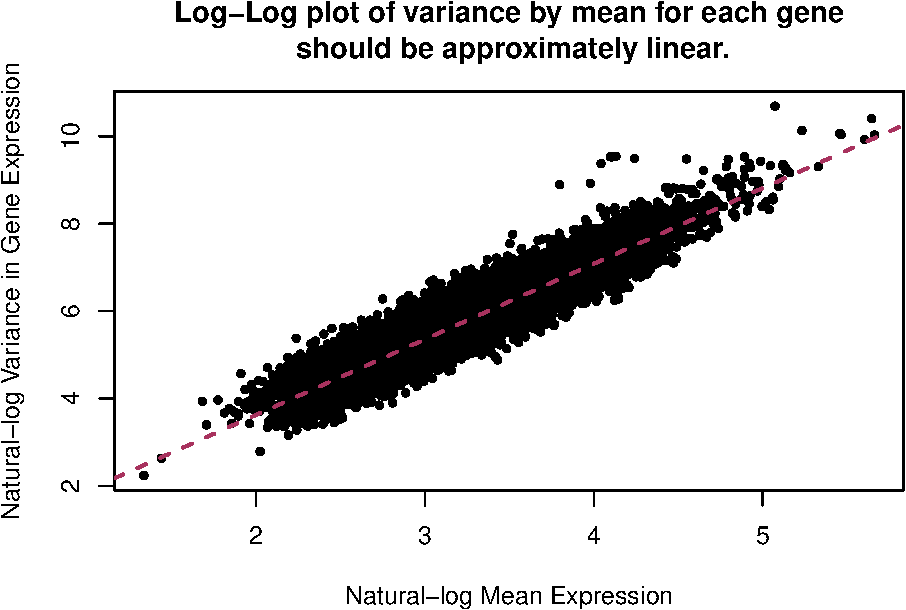
\includegraphics{DPFE_files/figure-latex/unnamed-chunk-13-1.pdf} We will
use the local VST function because it has the lowest standard deviation.

\begin{Shaded}
\begin{Highlighting}[]
\FunctionTok{runVST}\NormalTok{(dsgnObject, }\AttributeTok{blind =} \ConstantTok{FALSE}\NormalTok{, }\AttributeTok{fitType =} \StringTok{"local"}\NormalTok{, }\AttributeTok{makePlot =} \ConstantTok{TRUE}\NormalTok{, }\AttributeTok{writeTable =} \ConstantTok{FALSE}\NormalTok{, }\AttributeTok{writeRData =} \ConstantTok{TRUE}\NormalTok{)}
\end{Highlighting}
\end{Shaded}

\begin{verbatim}
## Scale for fill is already present.
## Adding another scale for fill, which will replace the existing scale.
## Scale for fill is already present.
## Adding another scale for fill, which will replace the existing scale.
\end{verbatim}

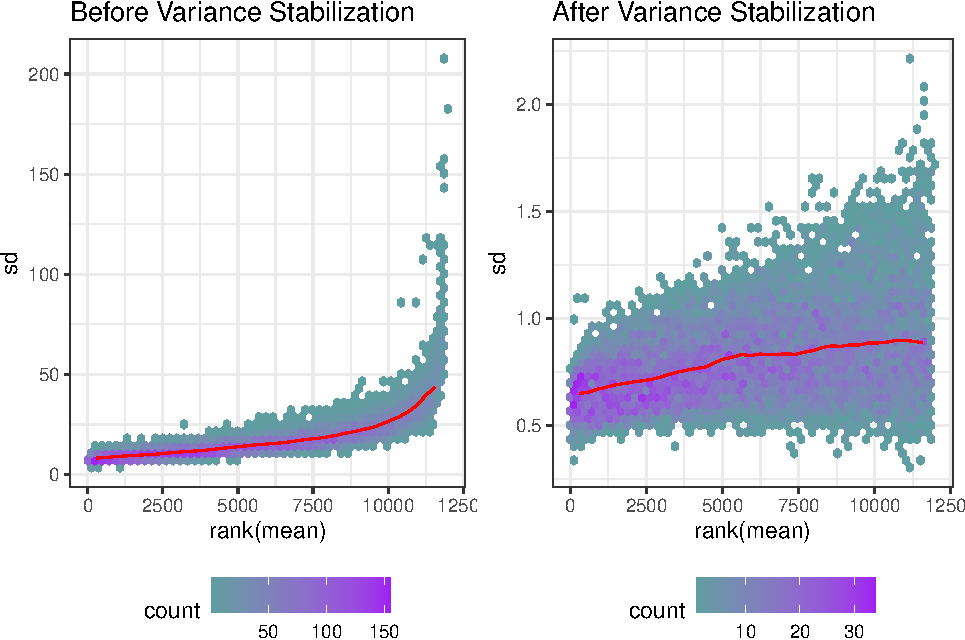
\includegraphics{DPFE_files/figure-latex/unnamed-chunk-14-1.pdf}

\begin{verbatim}
## class: DESeqTransform 
## dim: 11862 106 
## metadata(1): version
## assays(1): ''
## rownames(11862): 3155 _ 111 3816 _ 65 ... 3725 _ 108 3900 _ 10
## rowData names(6): baseMean baseVar ... dispGeneIter dispFit
## colnames(106): FD02 FD04 ... WYS03 WYS04
## colData names(8): Longitude Latitude ... Altitude sizeFactor
\end{verbatim}

\begin{Shaded}
\begin{Highlighting}[]
\CommentTok{\#runVST(dsgnObject, blind = FALSE, fitType = "mean", makePlot = TRUE, writeTable = FALSE, writeRData = FALSE)}

\CommentTok{\#runVST(dsgnObject, blind = FALSE, fitType = "rlog", makePlot = TRUE, writeTable = FALSE, writeRData = FALSE)}
\end{Highlighting}
\end{Shaded}

\begin{verbatim}
## [1] "After filtering, the number of genes remaining in the dataset are: 2470"
\end{verbatim}

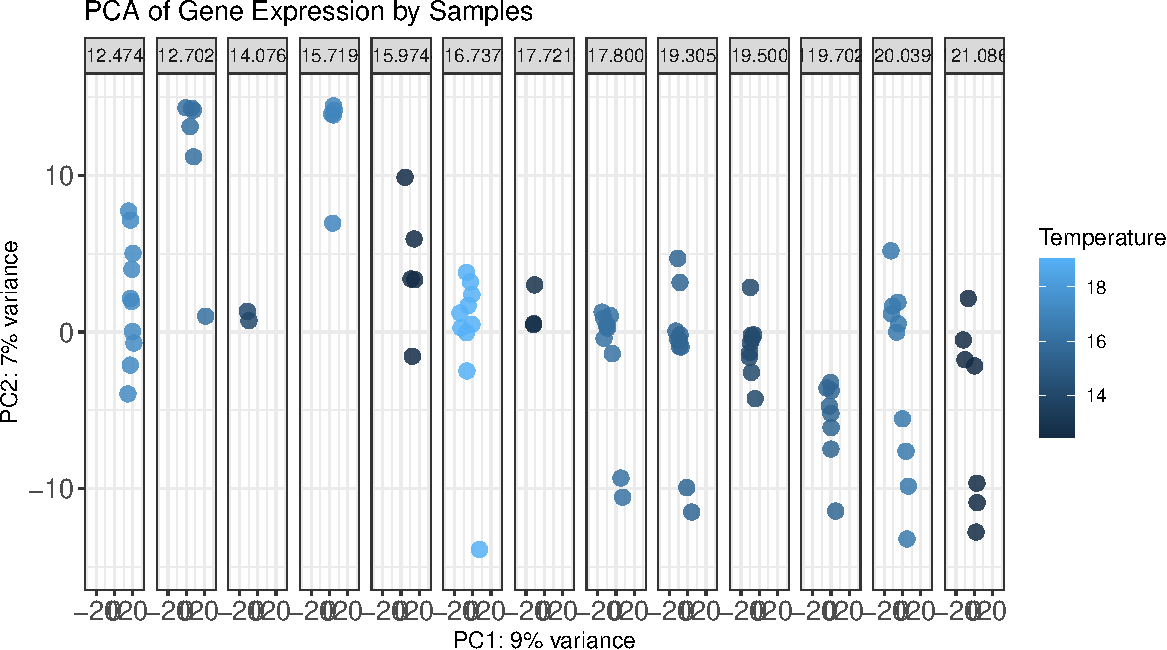
\includegraphics{DPFE_files/figure-latex/unnamed-chunk-17-1.pdf}

\begin{Shaded}
\begin{Highlighting}[]
\CommentTok{\#Install packages and load library}
\ControlFlowTok{if}\NormalTok{ (}\SpecialCharTok{!}\FunctionTok{requireNamespace}\NormalTok{(}\StringTok{"caret"}\NormalTok{, }\AttributeTok{quietly =} \ConstantTok{TRUE}\NormalTok{)) \{}
  \FunctionTok{install.packages}\NormalTok{(}\StringTok{"caret"}\NormalTok{)}
\NormalTok{\}}
\FunctionTok{library}\NormalTok{(caret)}
\end{Highlighting}
\end{Shaded}

\subsection{Discussion}\label{discussion}

While genetic data is harder to work with, the data preparation has
worked fairly well and given some very interesting and important
takeaways. Importantly, the variables being considered are all
numerical, which lends itself to different machine learning and feature
engineering approaches than mainly categorical data. It is clear that
the data benefited greatly from the variance stabilizing transformation,
as the raw counts had a standard deviation of over 200, while the VST
data was just over two, and with a much more stable spread. Principal
component analysis, at least the method I used, was not particularly
useful and may not be the best choice going forward. Additional feature
engineering may be required depending on the type of machine learning
model and how well the models perform.

\subsection{Next Steps}\label{next-steps}

The next step is to run some out-of-box machine learning models and
evaluate my choices so far. A random forest model, a support vector
machine, and a neural-network will all be trained on the training data
and tested on the test set. After the oob models are tested, other
techniques can be used to turn the hyperparameters of each model and
improve model accuracy. These techniques can include cross validation,
grid search, or elastic net.

\end{document}
